\chapter{Background subtraction}
\section{Assessing Beamline Contamination}
What is the beamline contamination? We define beamline contamination every TPC track matched to the WC track which is not a primary pion. There are 4 different types of beamline contaminations:
\begin{itemize}
\item[]1) electrons,
\item[]2) muons,
\item[]3) secondaries from pion events,
\item[]4) matched pile up events.
\end{itemize}

So, how do we handle this contamination?

The first step is to estimate what percentage of events used in the cross section calculation is not a primary pion.  
We estimate the percentage of electrons and muons in the beam via the beamline MC\footnote{Since the beamline composition is a function of the magnet settings, we simulate separately events for magnet current of -60A and -100A. 
We calculate the electron to pion and muon to pion ratio on the whole sample as the weighted sum of the corresponding ratio in the two current settings, 
\begin{equation}
\frac{N_e}{N_\pi}_{Data} = w_{60A}\frac{N_e}{N_\pi}_{60A}  + w_{100A}\frac{N_e}{N_\pi}_{100A},
\end{equation}
\begin{equation}
\frac{N_\mu}{N_\pi}_{Data} = w_{60A}\frac{N_\mu}{N_\pi}_{60A}  + w_{100A}\frac{N_\mu}{N_\pi}_{100A},
\end{equation}
where the weights $w_{60A}$ and $w_{100A}$ are the percentage of events in the corresponding magnet configuration passing the mass selection in data. }.
Once the beam composition is know,  we simulate the electrons, muons and pions with the DDMC and we subject the three samples to the same selection chain (WC2TPC match, shower filter, pile up filter, etc...). The percentage of electrons and muons surviving the selection chain is the  electron and muon contamination in the pion cross section sample.
The percentage of secondaries is given in the MC by the number of matched WC2TPC tracks which are not flagged as primary by Geant4.
We estimate the last type of contamination, the ``matched pile up" events, to be a negligible fraction, because of the definition of the WC2TPC match: we deem the probability of a single match with a halo particle in the absence of a beamline particle\footnote{ Events with multiple WC2TPC matches are always rejected.} extremely small.

\section{Subtraction}
Once we estimate the contaminants to primary pion ratio, the next step is subtracting their contribution from data for each type of contaminant independently. The contaminant samples are reconstructed and the corresponding interacting and incident histograms are produced. We then perform a bin by bin subtraction in the data interacting and incident histograms separately. A graphical rendering of this procedure is shown in Fig \ref{fig:backgroundSubtraction}
Once the data is background subtracted, we apply the correction laid out in the previous section.
\textcolor{blue}{How do we account for the error in the contamination subtraction? We change the electron/pion and muon/pion ratio and we see how much difference we get?}

\begin{figure}
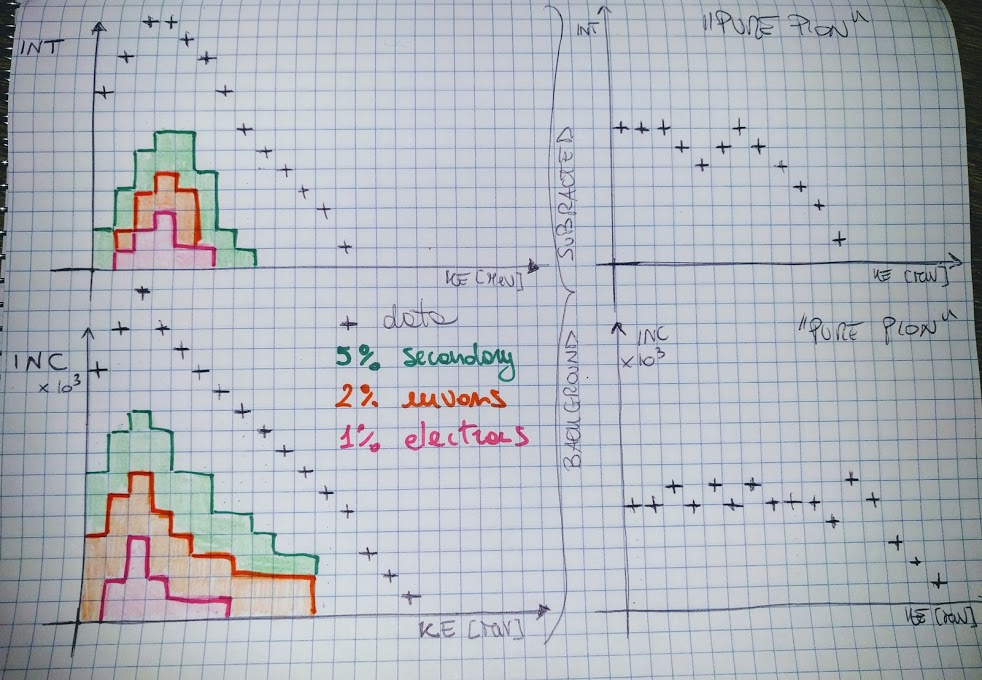
\includegraphics[width=\textwidth,height=\textheight,keepaspectratio]{Chapter-9/Images/FakePlot.jpg}
\label{fig:backgroundSubtraction}
\caption{A graphical rendering of the beamline contamination background subtraction. The contribution of the contaminants is shown in green for the secondaries, in orange for the muons and in pink for electrons. The colored plots are coming from the MC and are staggered. The percentages shown in the legend are the percentages of contaminants over the total number of events  passing the selection chain. We actually expect way less contamination.}
\end{figure}



